%%%%%%%%%%%%%%%%%%%%%%% file template.tex %%%%%%%%%%%%%%%%%%%%%%%%%
%
% This is a general template file for the LaTeX package SVJour3
% for Springer journals.          Springer Heidelberg 2010/09/16
%
% Copy it to a new file with a new name and use it as the basis
% for your article. Delete % signs as needed.
%
% This template includes a few options for different layouts and
% content for various journals. Please consult a previous issue of
% your journal as needed.
%
%%%%%%%%%%%%%%%%%%%%%%%%%%%%%%%%%%%%%%%%%%%%%%%%%%%%%%%%%%%%%%%%%%%
%
% First comes an example EPS file -- just ignore it and
% proceed on the \documentclass line
% your LaTeX will extract the file if required
\begin{filecontents*}{example.eps}
%!PS-Adobe-3.0 EPSF-3.0
%%BoundingBox: 19 19 221 221
%%CreationDate: Mon Sep 29 1997
%%Creator: programmed by hand (JK)
%%EndComments
gsave
newpath
  20 20 moveto
  20 220 lineto
  220 220 lineto
  220 20 lineto
closepath
2 setlinewidth
gsave
  .4 setgray fill
grestore
stroke
grestore
\end{filecontents*}
%
\RequirePackage{fix-cm}
%
%\documentclass{svjour3}                     % onecolumn (standard format)
%\documentclass[smallcondensed]{svjour3}     % onecolumn (ditto)
\documentclass[smallextended]{svjour3}       % onecolumn (second format)
%\documentclass[twocolumn]{svjour3}          % twocolumn
%
\smartqed  % flush right qed marks, e.g. at end of proof
%
\usepackage{graphicx}
\usepackage[numbers]{natbib}
\usepackage{geometry}
\usepackage{pdflscape}
%
\usepackage{mathptmx}      % use Times fonts if available on your TeX system
%
% insert here the call for the packages your document requires
%\usepackage{latexsym}
% etc.
%
% please place your own definitions here and don't use \def but
% \newcommand{}{}
%
% Insert the name of "your journal" with
\journalname{J Healthc Inform Res}
%
\begin{document}

\title{Identifying Effective Motivational Interviewing Sequences Using Automated Pattern Analysis
\thanks{This study was supported by a grant from the National Institutes of Health, NIDDK R21DK108071, Carcone and Kotov, MPIs.}
}
%\subtitle{Do you have a subtitle?\\ If so, write it here}

%\titlerunning{Short form of title}        % if too long for running head

\author{Mehedi Hasan, BS$^1$\and 
April Idalski Carcone, PhD$^2$\and 
Sylvie Naar, PhD$^3$\and 
Susan Eggly, PhD$^4$\and  
Gwen L. Alexander, PhD$^5$\and 
Kathryn E Brogan Hartlieb, PhD$^6$\and 
Alexander Kotov, PhD$^1$
}

%\authorrunning{Short form of author list} % if too long for running head

\institute{Alexander Kotov (corresponding author) \at
              5057 Woodward Suite 14001.6 \\
              Detroit, MI 48202\\
              Tel.: +1(313) 577-9307\\
              \email{kotov@wayne.edu} 
           \and
           $^1$Department of Computer Science, College of Engineering, Wayne State University, Detroit, MI 48202\\
$^2$Division of Behavioral Health Sciences, Department of Family Medicine and Public Health Sciences, Wayne State University School of Medicine, Detroit, MI 48202\\
$^3$Director, Center for Translational Behavioral Research, Department of Behavioral Sciences and Social Medicine, Florida State University, FL 32306\\  
$^4$Department of Oncology, Wayne State University/Karmanos Cancer Institute, Detroit, MI 48201\\
$^5$Department of Public Health Sciences, Henry Ford Health System, Detroit, MI 48202\\
$^6$Department of Humanities, Health and Society, Wertheim College of Medicine, Florida International University, Miami, FL 33199    
}

\date{Received: 12/03/2018 Revised: 04/15/2018 Accepted: }
% The correct dates will be entered by the editor


\maketitle

\begin{abstract}
Motivational Interviewing (MI) is an evidence-based strategy for communicating with patients about behavior change. Although there is strong empirical evidence linking “MI-consistent” counselor behaviors and patient motivational statements (i.e., “change talk”), the specific counselor communication behaviors effective for eliciting patient change talk are a subject of ongoing research. A significant barrier to this research is the time and resource-intensive cognitive tasks, including the manual coding and sequential analysis of coded transcripts, that are an integral part of the qualitative analysis of patient-counselor communication. Data mining and machine learning techniques have the potential to significantly reduce this barrier by partially automating these cognitive tasks. In this paper, we evaluate the empirical effectiveness of the Hidden Markov Model, a probabilistic generative model for sequence data, and closed frequent pattern mining, an algorithm used to mine the closed frequent patterns in MI communication sequences to inform MI practice. We conducted experiments with 1,360 communication sequences from 37 transcribed audio recordings of weight loss counseling sessions with African-American adolescents with obesity and their caregivers. Transcripts had previously been annotated with patient-counselor behavior codes using a specialized codebook. Empirical results indicate that Hidden Markov Model and closed frequent pattern mining techniques can identify meaningful and interpretable counselor communication strategies to guide clinical practice.

\keywords{sequential analysis \and hidden markov model \and closed frequent pattern mining \and motivational interviewing \and weight loss \and adolescents}
%\PACS{PACS code1 \and PACS code2 \and more}
% \subclass{MSC code1 \and MSC code2 \and more}
\end{abstract}

\section{Introduction}
\label{sec:intro}
Motivational Interviewing (MI) is an evidence-based strategy for communicating with patients about behavior change \citep{miller2013motivational}. The theory underlying MI’s clinical efficacy posits that behavior change is triggered by fostering an atmosphere of change, which is accomplished through the exercise of relational and technical skills \citep{miller2013motivational}. The relational hypothesis suggests that counselors’ use of accurate empathy, positive regard, and congruence create the “spirit of MI”, an optimal therapeutic state to explore behavior change. MI’s technical hypothesis \citep{miller2009toward} states that counselors’ use of communication techniques consistent with the MI framework (MICO; e.g., open-ended questions, reflections, advise with permission, affirmations, emphasize control, reframe, and support) will lead to patient “change talk”. Change talk are patient statements during clinical encounters that express their internal desire, ability, reasons, need for, and/or commitment to behavior change. Previous studies [3] have shown that change talk expressed during treatment sessions consistently predicts behavior change with results persisting as long as 34 months post-intervention [4]. In contrast, MI-inconsistent communication behaviors (MIIN; e.g., advising without permission, warning about behavioral consequences, and confronting) are hypothesized to lead to arguments against behavioral change and/or to maintain the status quo (referred to as counter change talk or sustain talk). Multiple studies have linked high rates of MICO to the expression of change talk and MIIN to sustain talk [5]. These studies have relied on session-level behavior counts and correlational analyses, which ignore the temporal order of utterances in patient-counselor communication, thereby limiting researchers’ ability to test MI’s technical hypothesis. 

Sequential analysis is an analytic approach to examine temporally ordered sequences of events or observations [6, 7]. Moyers and Martin [8] applied sequential analysis in a study of adults in treatment for alcohol abuse and found change talk was significantly more likely after MICO and sustain talk more likely after MIIN. A follow up study with the same population found change talk was more likely after two MICO behaviors, counselor questions about the positive and negative aspects of drinking and reflections of change talk, but these behaviors also led to sustain talk [9]. Surprisingly, MIIN was unrelated to sustain talk, but decreased the likelihood of change talk. Gaume et al. [10] used sequential analysis to study communication patterns during brief motivational interviewing for hazardous alcohol consumption with young adults conscripted into military service. They found MICO led to both change talk and sustain talk but the MIIN-to-sustain talk pattern was not observed. A second study with the same population confirmed that MICO leads to significantly more change talk and sustain talk [11]. In this sample, MIIN led to greater sustain talk, but was unrelated to change talk. Further analyses revealed that reflections were the only MICO behavior linked to increased change talk; reflections and other MICO behaviors, excluding questions, were related to increased sustain talk. Glynn and colleagues [12] linked reflections of change talk to the elicitation change talk and reflections of sustain talk to the elicitation of sustain talk among incarcerated adolescents with high rates of alcohol and marijuana use. In a study of adolescents engaged in weight loss treatment, Carcone et al. [13] used sequential analysis to identify three counselor behaviors likely to result in change talk: open-ended questions phrased to elicit change talk, reflections of change talk, and statements emphasizing decision-making autonomy. A parallel study of the adolescents’ caregivers [14] drew a similar conclusion, asking questions phrased to elicit change talk, reflections of change talk, and autonomy supportive statements were the counselor behaviors empirically linked to the elicitation of change talk. Across these studies, counselors’ use of reflections was consistently linked to change talk; other MICO behaviors led to change talk in some contexts but not others suggesting a need for additional research to understand the contexts in which the various MICO strategies are effective. 

The sequential analysis procedure used in the above MI process studies [8, 15-17] is based on the first-order Markov Chain model [8, 9, 11]. The Markov Chain model is a discrete-time stochastic process built on the assumption that the state of a system or condition changes over time and only depends on the previous event. Hence, Markov chain models have two main drawbacks. The first is their inability to preserve the long-range dependencies between observations in a sequence. However, in MI, an observed behavior can be influenced by any of the preceding behaviors. The second drawback is their inability to consider similarities between behavior codes and, consequently, their inability to identify multiple similar behaviors that lead to the same outcome. Thus, first-order Markov models may be insufficient to fully understand the associations between behaviors in patient-counselor communication sequences. Therefore, there is a need for more powerful computational methods, which consider clusters of behavior codes and long-term dependencies between behaviors, to identify causal relationships. The goal of the current research is to test the applicability of data mining methods to identify effective patterns of patient-counselor communication.

Several prior works have reported the results of adopting machine learning methods, such as topic models [18-22], classification methods [23-26] and neural networks [23, 27, 28] to the tasks of annotating MI transcripts and primarily for assessing intervention fidelity. Perez-Rosas et al. [25] developed a system to evaluate counselor fidelity to the MI framework by observing counselor language during motivational interviews. This system employed a support vector machine (SVM) classifier based on n-grams (contiguous sequences of words of a specified length), syntactic, and semantic features, which achieved nearly 90\% accuracy for predicting counselor questions and reflections. Patient’s engagement, verbal and non-verbal accommodation as well as topics discussed during the MI session, were analyzed to identify linguistic and acoustic features of counselor empathy. These features were then used to build a counselor empathy classifier that achieved an accuracy of up to 80\%. In our own recent work, we evaluated the accuracy of state-of-the-art classification methods and deep neural networks in conjunction with the lexical, contextual, and semantic features for the task of automated annotation of MI transcripts using codebooks with varying numbers of behavior codes [23]. The SVM model with the proposed features achieved 75\% accuracy for automated annotation of 17 behavior codes, which is comparable to human coders. In a follow up study [29], we applied Markov Models (MMs) and Recurrent Neural Networks (RNNs) to the classification of coded patient-counselor communication sequences into successful (sequences leading to patient change talk) and unsuccessful (sequences resulting in sustain talk). RNN achieved 87\% accuracy, 17\% greater than MMs (70\%) in predicting the success of motivational interviews. This paper represents the next phase in this line of research. We examine the efficacy of Hidden Markov Models (HMMs) and Frequent Pattern Mining in identifying the counselor communication strategies antecedent to patient change talk.

HMMs are widely used for the analysis of sequence data due to their ability to model short-range dependencies between clusters of discrete observations in a sequence. The HMM associates each observation in a sequence with a “hidden” state, where the hidden state corresponds to a different distribution over observations (i.e., distribution over behavior codes). Sequences of observations are modeled as transitions between different hidden states and sampling observations from each hidden state. HMMs were originally proposed for speech recognition [30], in which the states were used to represent all English language sounds. In biomedical informatics, HMMs were employed for the diagnosis of diseases and biological sequence modeling [31, 32]. For example, Doppler ultrasound was used to extract features from imaging data and then an HMM-based classifier was applied to distinguish healthy patients from those with heart disease [31], while HMM was used to capture important characteristics of protein families [32]. In the application of HMM to patient-counselor communication, hidden states correspond to sets of related behavior codes, such as a patient’s underlying motivational state, during a patient-counselor encounter. Although the MI literature has established patient change talk and commitment language (commitment language is a special class of change talk where patients express their intentions, plans, and action steps toward behavior change [33]) as the antecedents of patient’s behavior change [3], there is less clarity regarding which counselor communication strategies influence the articulation of change talk. Modeling successful and unsuccessful communication sequences during MI sessions with HMM can provide additional evidence to identify the counselor communication strategies that likely to lead to patient change talk and commitment language. 

Frequent pattern mining [34] is a class of data mining methods to identify sets of items (or observations, referred to as itemsets) which frequently appear together. Agrawal and Srikant [35] first introduced frequent pattern mining with the Apriori algorithm, which they developed to identify patterns in customer purchases. Since its introduction, frequent pattern mining has been applied to several other domains, including health informatics [36-39], medical imaging [37], chemical and biological analysis [40-42], web mining [43], and outlier analysis [44]. No published research has yet examined the utility of frequent pattern mining for studying patient-counselor communication. A major challenge in applying frequent pattern mining methods to patient-counselor communication sequences is the large number of resulting patterns, which include redundant patterns. To address this problem, we utilized the closed frequent itemset mining method [45], which produces less number of patterns in more compact form that are easier to interpret. In this study, we leveraged FPClose [46], an efficient state-of-the-art closed frequent pattern mining method, to identify the counselor behaviors that frequently lead to patient change talk. FPClose is the best closed frequent itemset mining algorithm, which shown highest performance in terms of running time and memory consumption.

In this paper, we focus on computational methods to facilitate the sequential analysis of MI transcripts to identify patterns of patient-counselor communication in successful and unsuccessful sequences in MI sessions. Analysis of these patterns provides empirical support for the specific counselor communication strategies that are effective at eliciting patient change talk. This knowledge will inform MI theory by providing additional evidence to support MI’s technical hypothesis. It will also inform clinical practice by facilitating the use of more effective and tailored counselor communication. This paper provides the first empirical evaluation of the effectiveness of closed frequent pattern mining to analyze patient-counselor communication sequences during MI sessions. Bertholet et al. [47] used HMM and adjusted regression models to examine the association of different sequences of “change talk” utterances with drinking outcomes in a brief motivational intervention. Their HMM model limited hidden states to three, which are "towards change", "away from change" and "non-determined". First and last hidden states decoded for a communication sequences, were used in conjunction with those three hidden states variables as predictors in a bivariate regression model, the results of which indicated that only the last state was significantly associated with drinking 12 months post-intervention. In the current study, we identified the optimal number of hidden states using HMM modeling of successful and unsuccessful sequences of patient-counselor communication. The goal of this study to evaluate the utility of using HMM and Frequent Pattern Mining to better understand the specific counselor communication strategies leading to patient change talk and sustain talk during Motivational Interviewing sessions. These two approaches offer the following advantages over the first-order Markov chain based methods most typically used in MI research. First-order Markov chain models identify the likely transitions between individual behaviors. In contrast, HMM summarizes transitions between clusters of related behavior codes (i.e., hidden states) allowing the identification of clusters of behaviors antecedent to change talk in successful patient-counselor communications and sustain talk in unsuccessful patient-counselor communications. Frequent pattern mining can identify patterns involving long-range dependencies between patient and counselor behaviors. Accounting for such long-range dependencies is important, since human behaviors, such as patient-counselor communication during MI sessions, are informed by all the antecedent behaviors and not just the immediately preceding behavior.

\section{Methods}
\label{sec:methods}
\subsection{Dataset}
\label{subsec:dataset}
The data set for this study consists of 37 transcripts from Motivational Interviewing (MI) sessions conducted with African American adolescents seeking weight loss treatment. Each transcript represented a one-on-one interaction between the adolescent patient and the MI counselor followed by a one-on-one interaction between the caregiver and the MI counselor. These encounters had previously been annotated using the Minority Youth Sequential Code for Observing Process Exchanges (MYSCOPE) [13]. The MYSCOPE is an adaptation of the original MI-SCOPE [48], a qualitative code scheme to characterize patient-counselor communication during MI treatment sessions. The MYSCOPE was informed by MI fidelity code schemes including the MI Treatment Integrity Scale (MITI) [49], the MI Skill Code (MISC) [50], and Amrhein’s conceptualization of change talk and commitment [51]. A primary coder used the MYSCOPE to annotate transcripts of all 37 sessions; a secondary coder coded 20\% (n = 7) of the sessions for inter-rater reliability which was good (k = .696). The experimental dataset consists of 7,192 patient, caregiver, and counselor utterances segmented and annotated with the MYSCOPE behavior codes, illustrated in Table~\ref{tab:codebook}.

% For tables use
\begin{table}
% table caption is above the table
\caption{MYSCOPE codebook.}
\label{tab:codebook}       % Give a unique label
% For LaTeX tables use
\begin{tabular}{lll}
\hline\noalign{\smallskip}
first & second & third  \\
\noalign{\smallskip}\hline\noalign{\smallskip}
number & number & number \\
number & number & number \\
\noalign{\smallskip}\hline
\end{tabular}
\end{table}

\subsection{Data preprocessing}
\label{subsec:datapreprocessing}
Utterances in MI session transcripts were segmented into successful and unsuccessful communication sequences. For each MI transcript, the stream of behavior codes from beginning to end was analyzed. Successful sequences were those that resulted in a patient change talk or commitment language statement and all preceding behavior codes were included. Unsuccessful sequences were similarly created for sequences resulting in sustain talk. A total of 1,360 sequences were generated. The majority of the sequences (n=1,102) were successful, which is expected for a treatment-seeking population, in which the initial motivation for behavior change is typically high. Successful sequences had an average length of 5.28 utterances, while unsuccessful sequences had on average 5.29 utterances. 

\subsection{Data Analysis}
\label{subsec:dataanalysis}
The Hidden Markov Model (HMM; implemented in the hmmlearn package which is publicly available at http://hmmlearn.readthedocs.io/en/latest/index.html) analysis aimed to identify clusters of related behavior codes within successful and unsuccessful communication sequences and to describe the relationships (transitions) between these clusters. Given a set of behavior code sequences, the posterior inference of HMM parameters involves the deduction of a temporal sequence of hidden states that best explains observations in each sequence. The emission probability matrix describes the distribution of observation symbols (i.e., the MYSCOPE behaviors displayed) for each hidden state and the transition probability matrix describes the transitions among the hidden states.

Training an HMM with a given number of hidden states (N) involves estimating the following parameters using the Baum-Welch algorithm:
M is the number of distinct observations symbols per state, i.e. the discrete codebook size (Table 1).
T is an  state transition probability matrix where  
E is an  matrix where , with observation symbol probability distribution for each state (emission probability matrix), and
p is the initial state distribution vector where .

In this study, two HMM models were trained, one using successful sequences and the other using unsuccessful sequences, with the objective of maximizing log-likelihood on the observed sequence. The optimal number of hidden states was determined by estimating the Bayesian information criterion (BIC) of HMM models with a different number of hidden states and selecting the model with the smallest BIC value, which indicates an optimal fit of HMM model. BIC minimizes negative log-likelihood but penalizes complexity (i.e. \# of hidden states), which is important for avoiding overfitting problem. HMM analyses suggested 5 hidden states was optimal for successful sequences and 2 hidden states were optimal for unsuccessful sequences (Figure~\ref{fig:bic}). 

% For two-column wide figures use
\begin{figure*}
% Use the relevant command to insert your figure file.
% For example, with the graphicx package use
  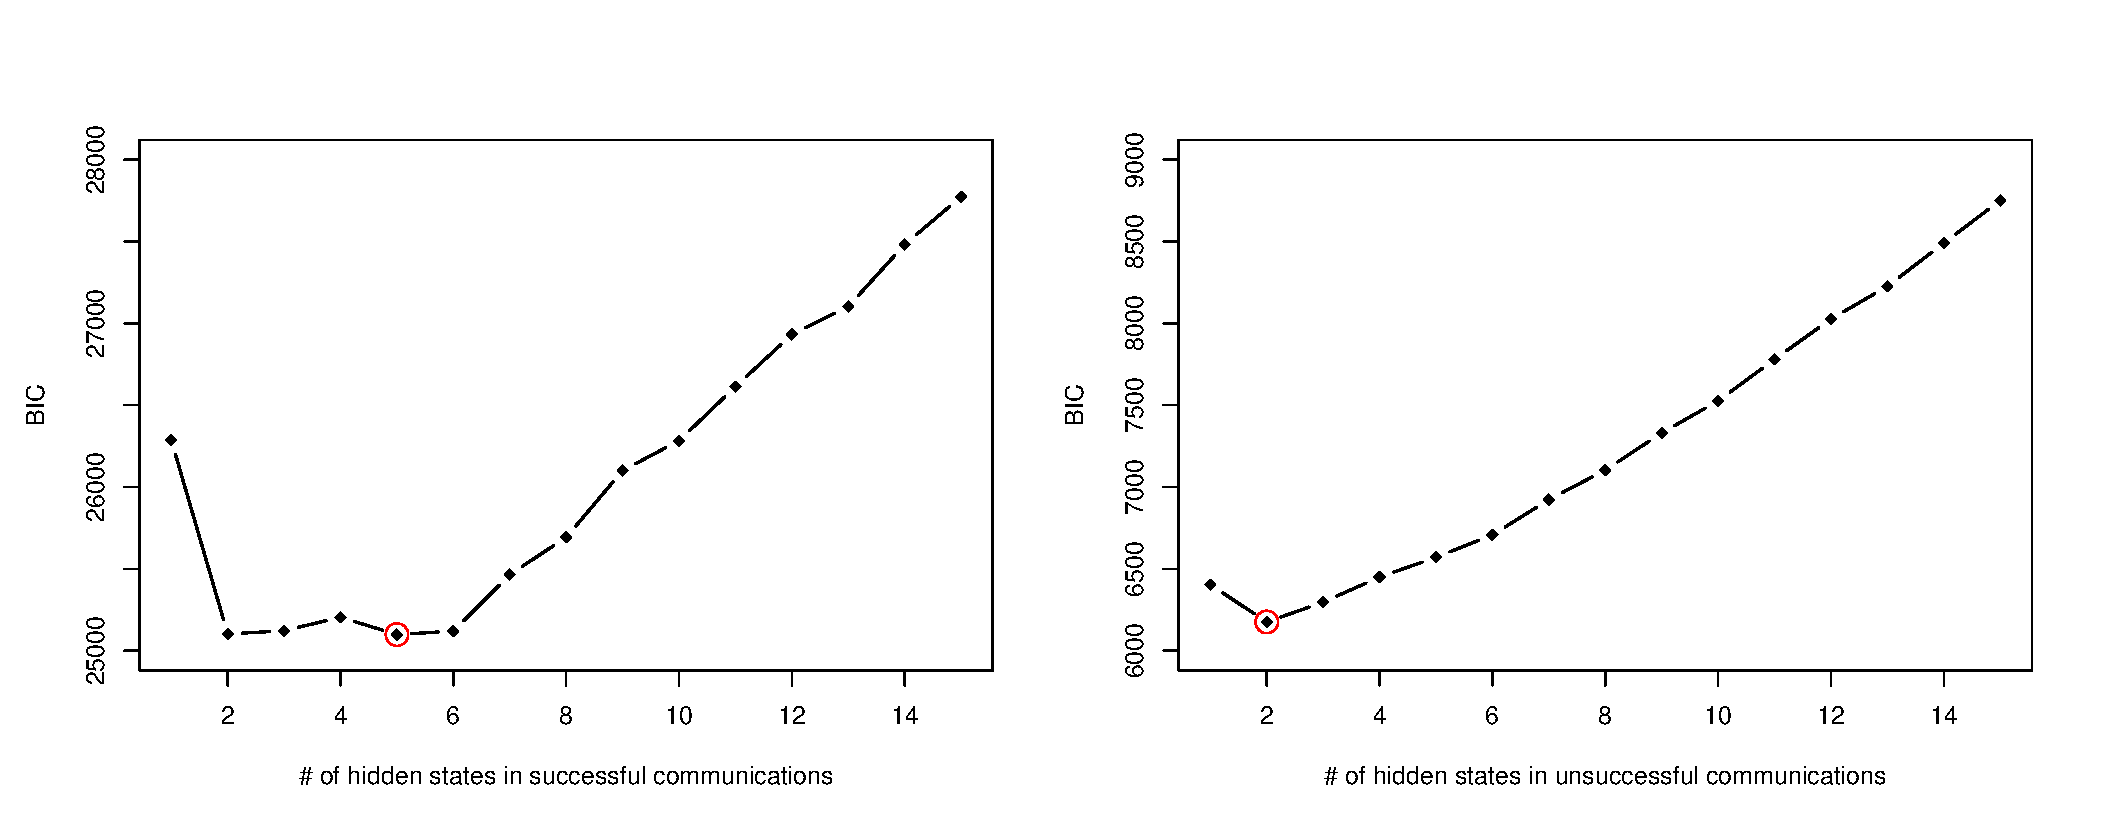
\includegraphics[width=1.0\textwidth]{figures/bic-vs-hidden-states.eps}
% figure caption is below the figure
\caption{Bayesian information criterion (BIC) of HMM models of successful (left) and unsuccessful (right) interviews by varying the number of hidden states.}
\label{fig:bic}       % Give a unique label
\end{figure*}

A second experiment was conducted with Frequent Pattern Mining. Orange3 and arules are two available pattern mining libraries implemented in python and r-programming, which support only a few pattern mining algorithms including frequent itemsets and association rules mining. However, we conducted our experiment using SPMF [52, 53], which offered more than 150 data mining algorithms. Moreover, SPMF is an open-source, fast and lightweight, a most popular and widely used Java-based data mining library. A frequent itemset is determined by surpassing a user-specified threshold called minimum support count\footnote{Support count: \# of times an itemset appears in the database}. For example, \{A\}, \{C\}, {D}, and {C, D} are frequent itemset in the database illustrated in Figure~\ref{fig:fpm}, because these itemsets appear at least 2 times which was the minimum support count identified in the example database. We reported closed frequent itemsets among all sequences of behavior codes in successful and unsuccessful sequences. A frequent itemset is closed if none of its supersets have the same support count [45], where a set X is a superset of another set Y if X contains all elements of the set Y. For example, the itemsets {A}, {C}, {D}, and {C, D} are not closed frequent itemsets because their supersets \{A, B\}, {B, C}, {B, D}, and {B, C, D} have the same number of support. Therefore, {B}, {A, B}, {A, D}, {B, C}, {B, D}, and {B, C, D} are closed frequent itemsets because none of their supersets have same the number of support count. On the other hand, {A, C}, {A, B, C}, {A, B, D}, {A, C, D} and {A, B, C, D} have support count 1, 0, 1, 0, and 1, respectively, which are less than minimum support count and identified as non-frequent itemsets. This study applied FPClose [46], an efficient close frequent pattern mining algorithm in SPMF, to identify frequent patient-counselor behaviors in MI communication sequences. To improve the model’s ability to identify frequent patient behaviors, FPClose [46], a FP-tree based algorithm [54, 55] was used. FPClose identifies closed frequent itemsets by utilizing an FP-tree data structure in combination with the FP-array technique to avoid the frequent traversal of FP-trees. Before applying the FPClose method, the dataset was transformed into the expected format used by the algorithm in the SPMF library. Minimum support threshold is a certain proportion having a meaningful representation of patterns determined by the domain expert. Since there is no standard for the selection of minimum support threshold, by following the studies [56-57], the minimum support count considered was 10\% of the total number of sequences which is 110 for successful and 25 for unsuccessful sequences. In our study, support counts representing ≥10\% of the patterns was the threshold for the result interpretation. 

% For two-column wide figures use
\begin{figure*}
% Use the relevant command to insert your figure file.
% For example, with the graphicx package use
  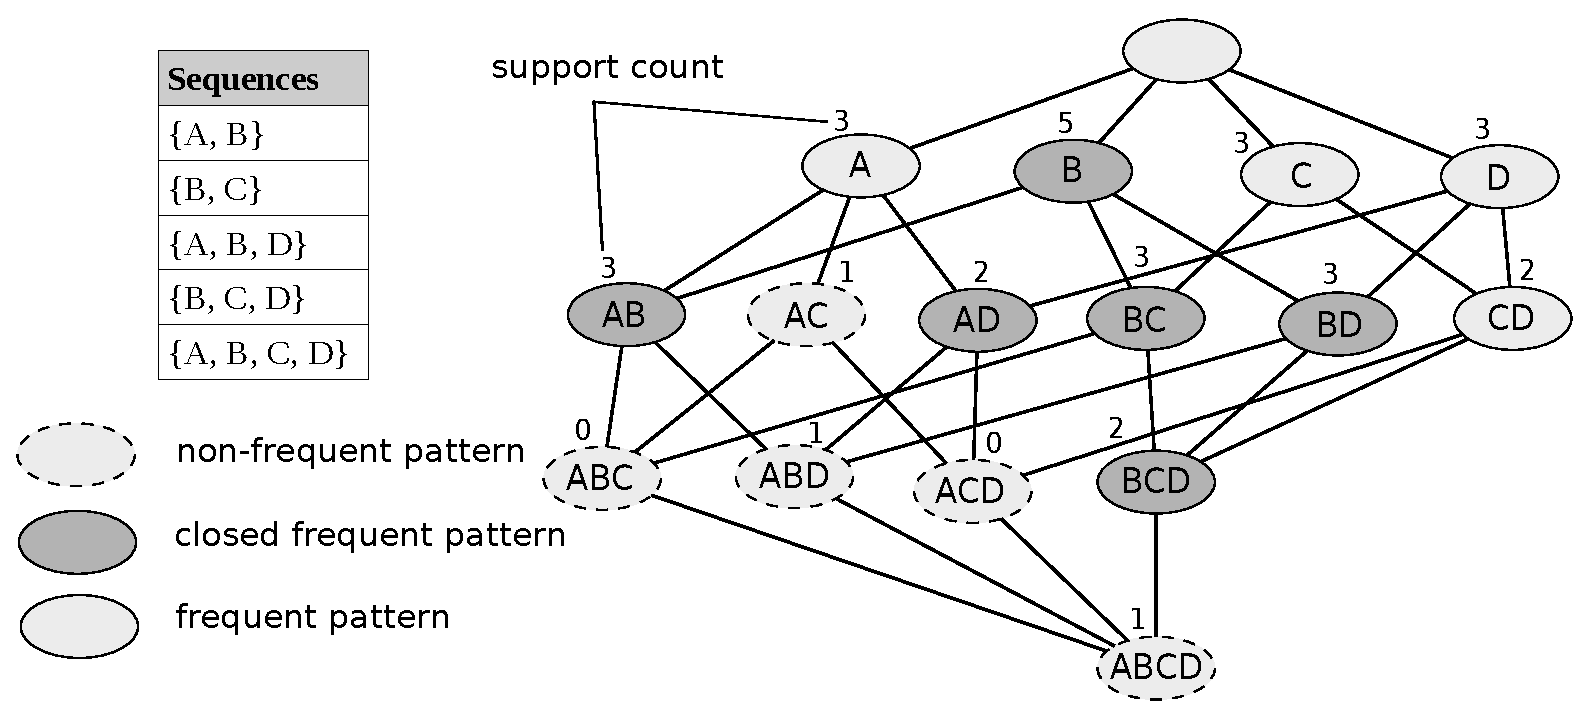
\includegraphics[width=0.95\textwidth]{figures/fpm.eps}
% figure caption is below the figure
\caption{Different type of itemsets is illustrated with a frequent pattern mining method applied on transaction database by considering minimum support count 2, where TID represents the transaction ID of the corresponding items.}
\label{fig:fpm}       % Give a unique label
\end{figure*}


\section{Results}
\label{sec:results}
The transition and emission probability matrices of HMM model, are reported in Tables~\ref{tab:transition} and~\ref{tab:emission}. The three behaviors with the highest frequency, representing 45-69\% of each state’s emission transitions, were used to interpret the emission matrix and label the hidden states. Most (84\%) successful sequences began in a state characterized as “high motivation” as evidenced by a greater proportion of three counselor behaviors: reflections of change talk (29\%), reflections of commitment language (17\%), and affirmations (12\%). Successful sequences began in a state of “high receptivity” 11\% of the time. “High receptivity” sequences were characterized by nearly equal proportions of information offered using patient-centered strategies (18\%), questions to elicit change talk (16\%), and affirmations (15\%). Few successful sequences began in states of “moderate receptivity” and “low receptivity” (2\% and 3\% of the time, respectively). These two states were characterized by different proportions of the same behaviors. Moderate receptivity sequences were distinguished from low receptivity sequences by a greater proportion of counselor questions to elicit change talk (20\% versus 11\%) and a lower proportion of patient low uptake statements (16\% versus 28\%); counselor statements emphasizing the patient’s autonomy were about the same (14\% versus 17\%). No (0\%) successful sequence began in the “active feedback” state, which was characterized by three patient behaviors, low uptake (47\%), weight-related high uptake (12\%), and other-related high uptake (10\%). Successful sequences transitioned from “high motivation” to “active feedback” most often (41\%). “active feedback”, in turn, most frequently transitioned to “high receptivity” (39\%). The “moderate receptivity” state transitioned to most often to “active feedback” (27\%) and automatically transitioned back to “moderate receptivity” (24\%) or to “low receptivity” (23\%) with similar frequency. The full transition matrix is presented in Table~\ref{tab:transition}.

In contrast, the majority of unsuccessful sequences (98\%) began in a state of “ambivalence” as indicated by the greater proportion of counselor reflections of both change talk (20\%) and sustain talk (12\%) as well as affirmations (13\%). About 2\% of the time unsuccessful sequences started in a state of “avoidance”. Higher rates of patient low uptake (29\%) and other-related high uptake (11\%) statements, and counselor patient-centered information (18\%) distinguished “avoidant” sequences. Both “ambivalent” (84\%) and “avoidant” (61\%) states most frequently transitioned to the “avoidant” state.


%\newgeometry{margin=2cm} % modify this if you need even more space
\begin{landscape}
% For tables use
\begin{table}
% table caption is above the table
\caption{Hidden Markov Model Emission Matrices}
\label{tab:emission}       % Give a unique label
% For LaTeX tables use
\begin{tabular}{lll}
\hline\noalign{\smallskip}
first & second & third  \\
\noalign{\smallskip}\hline\noalign{\smallskip}
number & number & number \\
number & number & number \\
\noalign{\smallskip}\hline
\end{tabular}
\end{table}

% For tables use
\begin{table}
% table caption is above the table
\caption{Hidden Markov Model Transition Matrices}
\label{tab:transition}       % Give a unique label
% For LaTeX tables use
\begin{tabular}{lll}
\hline\noalign{\smallskip}
first & second & third  \\
\noalign{\smallskip}\hline\noalign{\smallskip}
number & number & number \\
number & number & number \\
\noalign{\smallskip}\hline
\end{tabular}
\end{table}

\end{landscape}
\restoregeometry


Frequent communication patterns in successful and unsuccessful patient-counselor communication sequences are shown in Table~\ref{tab:patterns}. Results from frequent pattern mining analysis indicate that reflections of change talk were the most frequent counselor communication behavior in both successful (36.1\%) and unsuccessful sequences (33.7\%). For each pattern, the significance of difference between successful and unsuccessful communications was reported by computing p-value using Pearson chi-square test. Successful sequences were distinguished from unsuccessful sequences by a higher frequency of counselor questions phrased to elicit change talk (30.8\% versus 17.4\%, p<0.0001), statements emphasizing the patient’s decision-making autonomy (28.5\% versus 18.6\%, p=0.0012), questions phrased to elicit commitment language (18.1\% versus 11.6\%, p=0.0118), and reflections of commitment language (20.7\% versus 15.1\%, p= 0.0423). In contrast, unsuccessful sequences were characterized by greater frequency of questions to elicit perceived barriers (14.7\% versus 0\%, p= <0.0001), reflections of sustain talk (27.1\% versus 15.8\%, p=<0.0001), providing information (28.7\% versus 22.1\%, p= 0.0254) and other reflections (11.6\% versus 0\%, p=<0.0001). In 14.0\% of the successful sequences, reflections of change talk were paired with a question phrased to elicit change talk; this pattern did not appear in unsuccessful sequences. In contrast, in 10.5\% of the unsuccessful sequences, reflections of change talk were paired with information; this pattern did not appear in successful sequences.

% For tables use
\begin{table}
% table caption is above the table
\caption{Frequent communication patterns in successful and unsuccessful patient-counselor communication sequences.}
\label{tab:patterns}       % Give a unique label
% For LaTeX tables use
\begin{tabular}{lll}
\hline\noalign{\smallskip}
first & second & third  \\
\noalign{\smallskip}\hline\noalign{\smallskip}
number & number & number \\
number & number & number \\
\noalign{\smallskip}\hline
\end{tabular}
\end{table}

\section{Discussion}
\label{sec:discussion}
We present the application of HMM and frequent pattern mining to test the technical hypothesis guiding Motivational Interviewing which suggests that counselors use of “MI-consistent” communication strategies (MICO) will lead to patient change talk [2]. Previous studies have empirically linked counselors’ use of MICO to higher rates of patient change talk in first-order Markov Chain models [8, 9, 11]. Evidence from the current study using machine-learning methods of pattern analysis provides stronger evidence for MI’s technical hypothesis by considering longer-term dependencies in the data. Both HMM and frequent pattern mining consider behavioral antecedents beyond the counselor behavior immediately preceding a patient change talk statement offered by simple first-order Markov chain models. The ability of HMM and frequent pattern mining to identify critical patterns in patient-counselor communication sequences advances research in the field of Motivational Interviewing which has previously relied upon simple Markov chain models [8-14].

The states identified in HMM model, were given labels to describe the underlying “state” of the MI session. These labels were based on an analysis and interpretation of the three behaviors with the highest frequency according to the emission matrix. Three behaviors were interpreted because together they represented 45-69\% of the behaviors associated with a given state and all represented at least 10\%. These labels made it easier to understand types of interactions occurred between counselors and patients. 

In both analyses, MICO communication strategies were characteristic of successful sequences (i.e., those resulting in a change talk statement). In HMM, the majority successful sequences began in the high motivation state where counselors frequently used reflections of change talk or commitment language and affirmations. Other high frequency counselor behaviors observed in successful sequences included statements emphasizing patients’ decision-making autonomy, questions phrased to elicit change talk, and the provision of information using patient-centered strategies. The frequent pattern mining results were similar. Reflections of change talk was the most frequent counselor communication strategy in successful sequences, followed by open questions phrased to elicit change talk, affirmations, statements emphasizing the patient’s decision-making autonomy, and sensitively provided information. Previous MI sequential analysis studies using first-order Markov chain models to analyze communication sequences have linked patients’ expression of change talk to counselor reflections of change talk, [9, 11-14] open questions phrased to elicit change talk, [9, 13, 14], and statements emphasizing the patient’s decision-making autonomy [13, 14]. These studies did not find a link between change talk and counselors’ use of affirmations or the provision of information when examined independently of the MICO index. Thus, the current study is the first to provide empirical evidence for these causal linkages. One reason for this unique finding may be the treatment context, adolescent patients engaged in a voluntary weight loss trial. Adaptations of MI for the health care setting suggest that asking questions, demonstrating active listening through reflections, and the provision of information are critical communication skills for encouraging health-related behavior change [58]. Thus, providing information in a patient-centered manner in the context of health care treatment may be necessary to ensure patients have the requisite knowledge of their health care problem and its treatment. 

The analysis of unsuccessful sequences, i.e., those resulting in a patient sustain talk statement, was typified by a combination of MICO and MI-inconsistent communication strategies (MIIN). Specifically, the majority of unsuccessful sequences in the HMM analysis began in a state of Ambivalence which was characterized by large proportions of counselor reflections of both change talk and sustain talk. Similarly, in the frequent pattern mining analysis of unsuccessful sequences, reflections of change talk and sustain talk were two of the three most frequent counselor behaviors observed. These results are consistent with those of Gaume and colleagues [11] who found both MICO and MIIN were linked to the elicitation of sustain talk in a sample of at-risk young adult drinkers enlisted into the military. Specifically, counselors’ use of simple and complex reflections and “other MICO” behaviors (an index of affirmations, statements emphasizing patient control, reframing, and support) were empirically linked to the elicitation of sustain talk; neither open or closed questions were related to the elicitation of sustain talk. Carcone et al [13] found counselors’ questions and reflections specifically phrased to elicit patient sustain talk were the counselor behaviors most likely to elicit sustain talk among adolescents engaged in a weight loss trial. In contrast, Moyers et al. [9] found questions about the positive and negative aspects of the target behavior and reflections of sustain talk were empirically linked to the elicitation of sustain talk but MIIN was not. These variable findings provide further support for the need to tailor the communication strategies MI counselors use to the treatment context. 

This study is part of a line of research to develop machine-learning models to annotate (code) and analyze patient-counselor communication patterns. We have previously reported on the development of a model to annotate clinical transcripts [18, 21, 23]. Experiments applying the annotation model to novel datasets are underway to assess the generalizability of the model to more diverse types of clinical encounters (e.g, email coaching to increase fruit and vegetable intake, HIV clinical care visits). In this study, we present the next phase of this research, the sequential analysis of patient-counselor communication data to identify the counselor communication strategies linked to the elicitation of change talk and sustain talk. Next steps include examining the performance of these models in diverse data sets representing different populations and behavioral problems. We are also experimenting with machine learning methods to segment (parse) the stream of communication behavior into chunks representing a patient or counselor utterance to which the annotation model can then assign a behavior code. Together, these models form the basis of a complete system to automatically code and analyze patient-counselor interactions. An automated system for behavioral coding and analysis could substantially accelerate the pace of research on the causal mechanism of Motivational Interviewing which informs theory and clinical practice by providing clinicians with information about how to best tailor their communication strategies with discrete patient populations.
 
This study is limited by the use of one dataset composed of 37 Motivational Interviewing transcripts of counseling sessions with African American adolescents in weight loss treatment. Thus, there is a need to replicate these findings with larger and more diverse data samples as the findings may not be representative of communication patterns in other contexts employing the Motivational Interviewing framework. In fact, when interpreted in light of the published literature, the results obtained in these experiments suggest that communication patterns are likely to vary given the treatment context. There are, however, consistencies with previous Motivational Interviewing process studies providing support for the validity of our findings and suggesting some counselor communication strategies may cut across treatment contexts. Next steps for this work include enhancing the performance and utility of machine learning models for sequential analysis by combining transcript annotation with sequential analysis. Another limitation of this work is the fact that successful and unsuccessful sequences were analyzed independently. One implication of this approach is that the utility of a counselor behavior, such as the provision of information, to shift an interaction destined for unsuccess to one of success cannot be determined from these analyses.

\section{Conclusion}
\label{sec:conclusion}
These results add to the growing evidence base examining the mechanisms of effect in Motivational Interviewing using modeling approaches that overcome critical shortcomings of previous methods. While counselors’ use of “MI-consistent” communication behaviors has been previously linked to higher rates of change talk in correlational studies [8, 15-17] and simple Markov chain models [8, 9, 11]. The use of HMM and frequent pattern mining analyses improves upon these approaches by considering long-term dependencies in the data. The results of this work suggest a more complex pattern between counselor communication behaviors and patient talk that varies depending on the context in which Motivational Interviewing is being used. 

\section{Conflict of Interest}
\label{sec:conflictofInterest}
On behalf of all authors, the corresponding author states that there is no conflict of interest.

%Text with citations \citep{wei2006semi} and \citep{keogh2000scaling}.

%\paragraph{Paragraph headings} Use paragraph headings as needed.
%\begin{equation}
%a^2+b^2=c^2
%\end{equation}

\begin{acknowledgements}
We would like to thank the student assistants in the Department of Family Medicine and Public Health Sciences at Wayne State University School of Medicine for their help in developing the training dataset. The authors would like to thank Lisa Todd, JD, MA for her thoughtful feedback and clinical expertise in the interpretation of these data.
\end{acknowledgements}

% BibTeX users please use one of
%\bibliographystyle{spbasic}      % basic style, author-year citations
%\bibliographystyle{spmpsci}      % mathematics and physical sciences
\bibliographystyle{natbib}       % JHIR format
%\bibliographystyle{spphys}       % APS-like style for physics
\bibliography{references}   % name your BibTeX data base

\end{document}
% end of file template.tex

